\section{Kết quả thực nghiệm và thảo luận}
\label{sec:results}

\subsection{Khảo sát có kiểm soát các bộ lọc và phân ngưỡng tạo ứng viên}
\label{subsec:bench_filters}
Giai đoạn đầu tiên quyết định chất lượng của tập ứng viên $\{\Omega_i\}$: nếu bộ lọc không đủ mạnh, nhiễu đốm sẽ tạo ra hàng chục vùng vụn; ngược lại, nếu làm mượt quá mức, các dải dầu hẹp sẽ bị xóa nhòa. Chúng tôi tiến hành khảo sát thực nghiệm có kiểm soát 13 cấu hình lọc không gian kết hợp phân ngưỡng toàn cục Otsu (cố định ngưỡng diện tích $A_{\min} = 16$ pixels) trên toàn bộ $671$ ảnh thuộc tập kiểm định (Validation).

\begin{figure*}[!t]
\centering
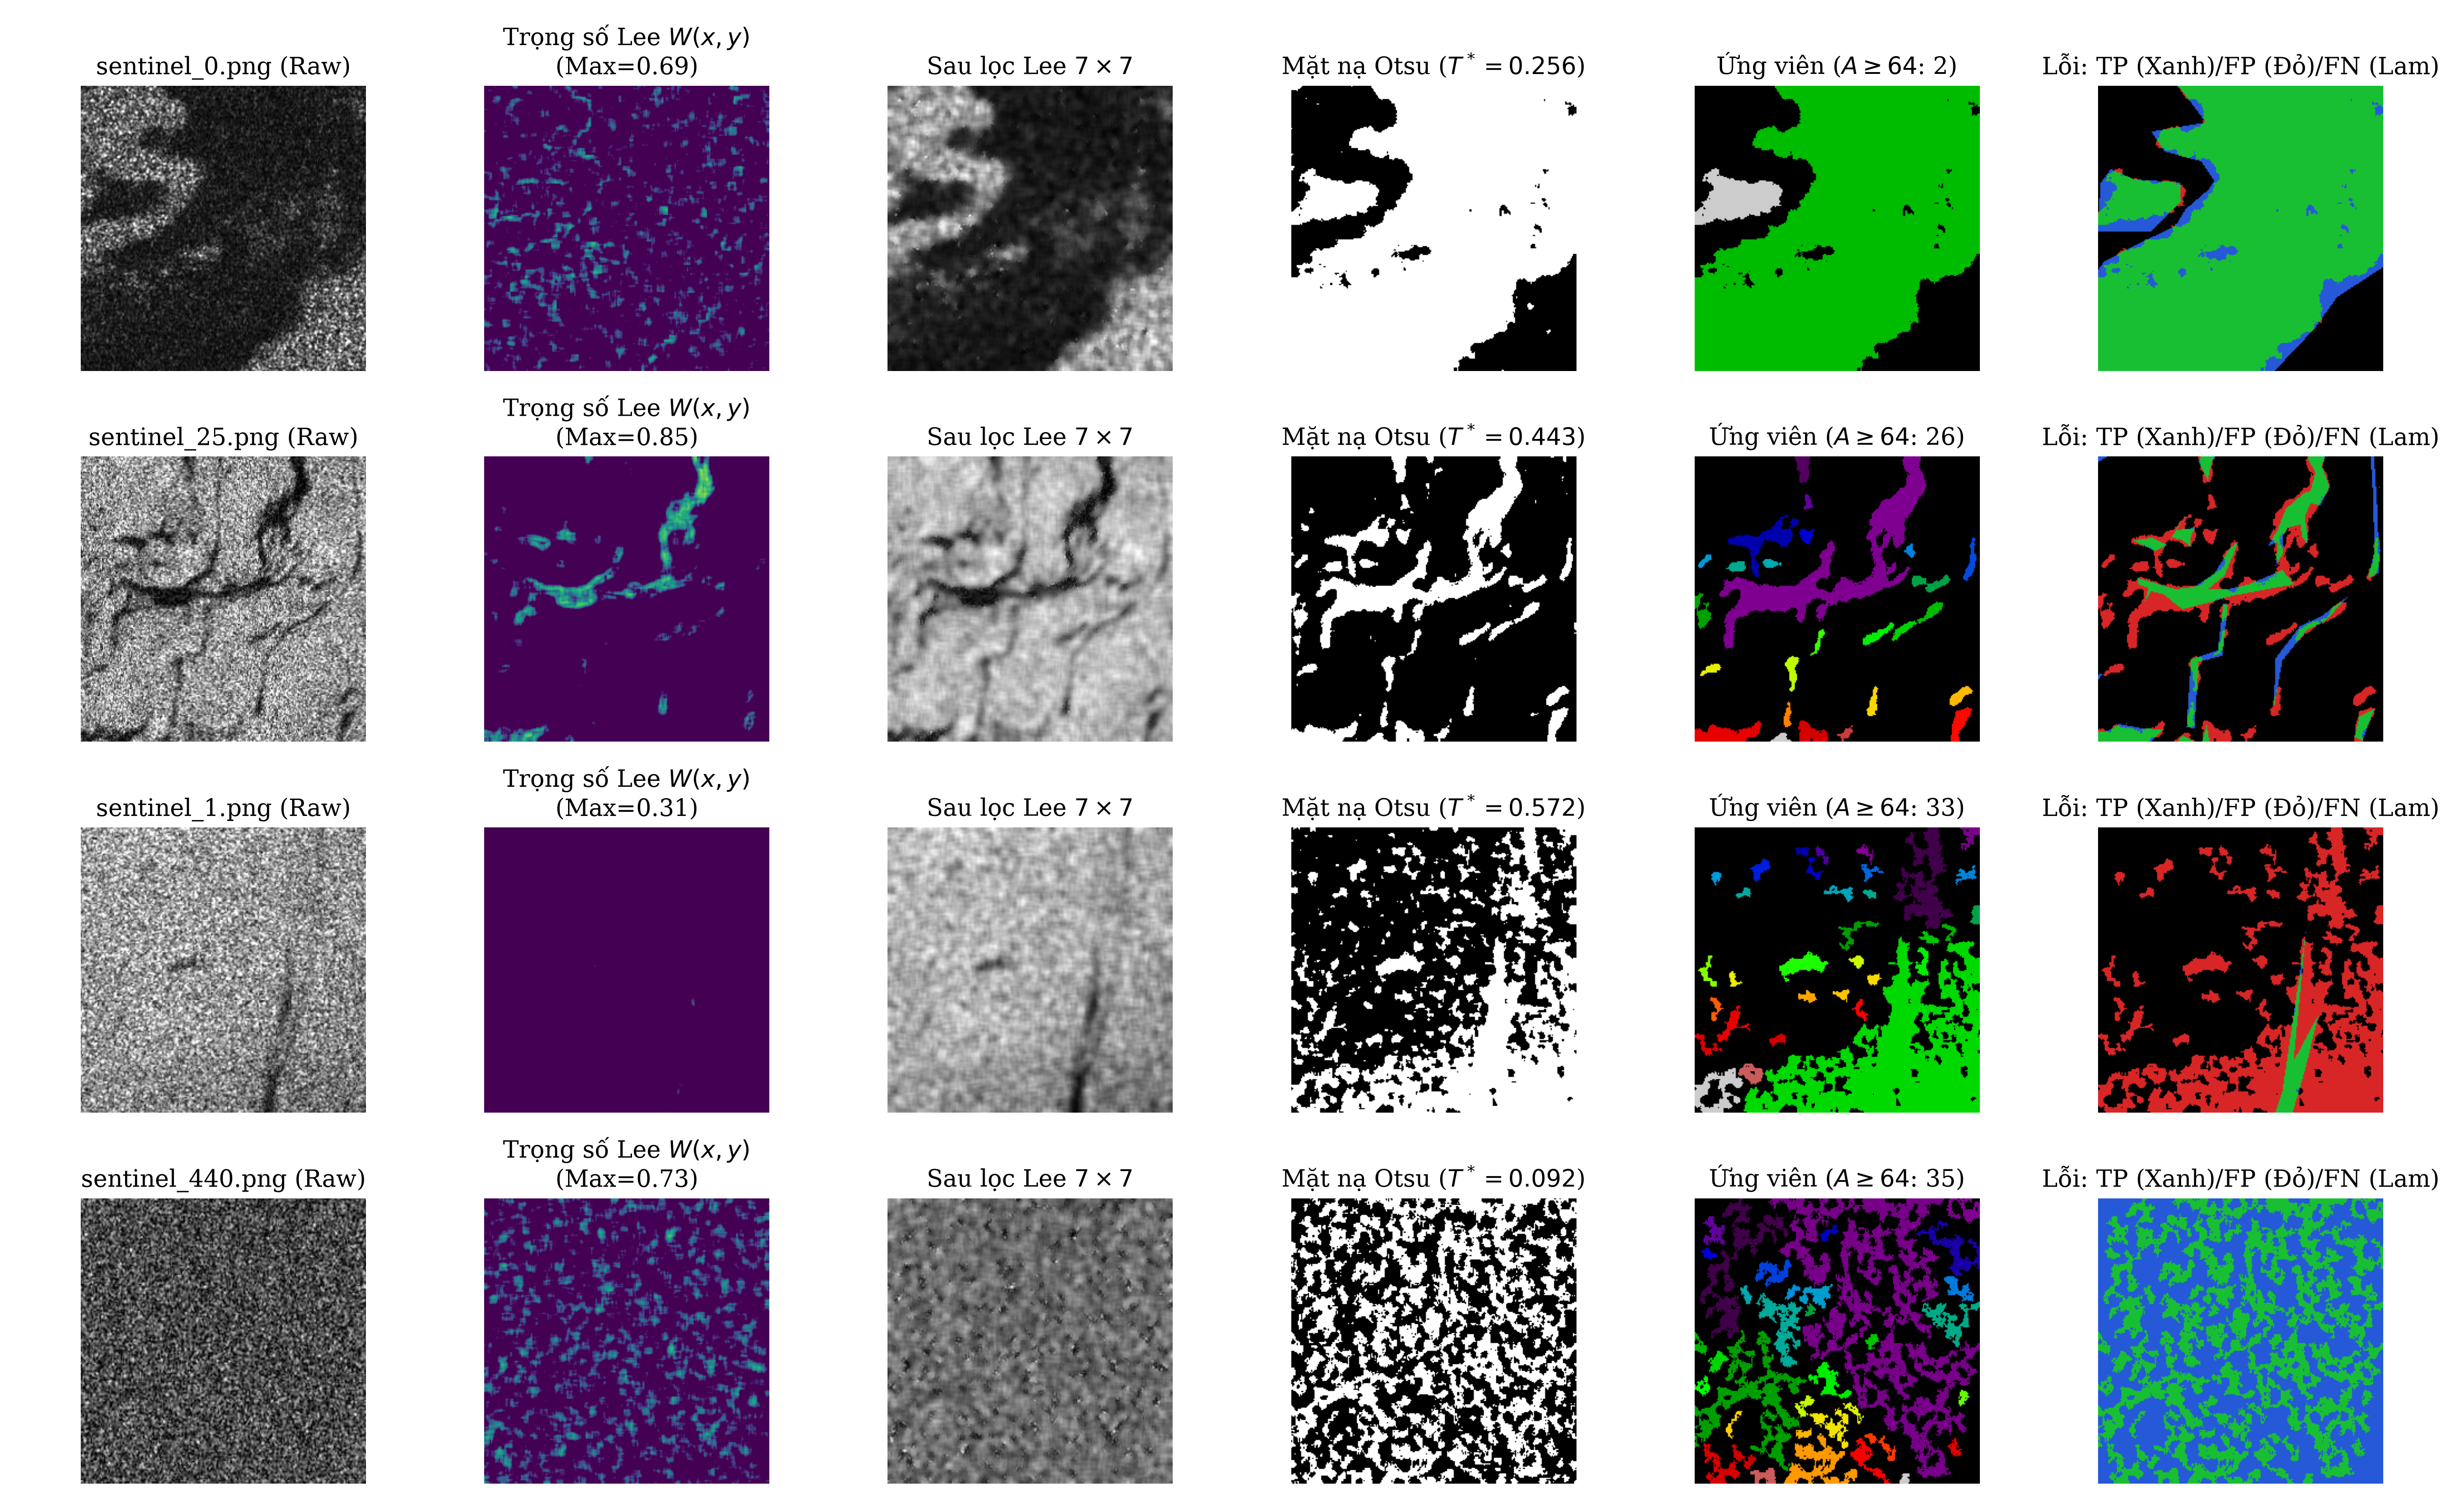
\includegraphics[width=\textwidth]{figures/fig3_step_by_step_pipeline.png}
\caption{Trực quan hóa các bước biến đổi trung gian của quy trình trên 4 cảnh SAR đại diện (\texttt{val/sentinel\_0.png}, \texttt{val/sentinel\_25.png}, \texttt{val/sentinel\_1.png}, \texttt{val/sentinel\_440.png}): Ảnh thô $\to$ Bản đồ trọng số Lee $W(x, y)$ $\to$ Ảnh sau lọc Lee $7 \times 7$ $\to$ Mặt nạ nhị phân Otsu $\to$ Vùng ứng viên sau lọc diện tích $A \ge 64$ $\to$ Bản đồ phân loại lỗi cấp điểm ảnh (True Positive: Xanh lá, False Positive: Đỏ, False Negative: Lam).}
\label{fig:step_pipeline}
\end{figure*}

\begin{table*}[!t]
\centering
\caption{So sánh có kiểm soát 13 cấu hình lọc không gian (cố định phân ngưỡng Otsu, $A_{\min} = 16$) trên toàn bộ 671 ảnh tập kiểm định (Validation). Khoảng tin cậy Bootstrap 95\% của $\Delta\text{F1}$ được tính qua $2\,000$ lần lấy mẫu lại có hoàn lại theo patch.}
\label{tab:filter_benchmark}
\resizebox{\textwidth}{!}{%
\begin{tabular}{lcccccccc}
\toprule
\textbf{Cấu hình bộ lọc} & \textbf{TP} & \textbf{FP} & \textbf{FN} & \textbf{Prec} & \textbf{Rec} & \textbf{Cand F1} & \textbf{Pix IoU} & \textbf{$\Delta\text{F1}$ vs.\ Lee $7\times 7, L=4$ (95\% CI)} \\
\midrule
\textit{None (Không lọc)} & 518 & $39\,283$ & $2\,222$ & 0.0130 & 0.1891 & 0.0244 & 0.4272 & $+0.0612 \quad [+0.0534, +0.0693]$ \\
\textit{Median $3 \times 3$} & 758 & $50\,479$ & $1\,982$ & 0.0148 & 0.2766 & 0.0281 & 0.4780 & $+0.0574 \quad [+0.0508, +0.0645]$ \\
\textit{Median $5 \times 5$} & 910 & $36\,046$ & $1\,830$ & 0.0246 & 0.3321 & 0.0458 & 0.5241 & $+0.0397 \quad [+0.0346, +0.0451]$ \\
\textit{Gaussian $\sigma = 0.8$} & 794 & $47\,039$ & $1\,946$ & 0.0166 & 0.2898 & 0.0314 & 0.4849 & $+0.0541 \quad [+0.0476, +0.0608]$ \\
\textit{Gaussian $\sigma = 1.2$} & 895 & $40\,877$ & $1\,845$ & 0.0214 & 0.3266 & 0.0402 & 0.5118 & $+0.0453 \quad [+0.0398, +0.0513]$ \\
\textit{Lee $3 \times 3$ ($L=1$)} & 821 & $46\,341$ & $1\,919$ & 0.0174 & 0.2996 & 0.0329 & 0.4909 & $+0.0526 \quad [+0.0462, +0.0592]$ \\
\textit{Lee $3 \times 3$ ($L=4$)} & 822 & $46\,897$ & $1\,918$ & 0.0172 & 0.3000 & 0.0326 & 0.4907 & $+0.0529 \quad [+0.0466, +0.0595]$ \\
\textit{Lee $5 \times 5$ ($L=1$)} & 961 & $32\,247$ & $1\,779$ & 0.0289 & 0.3507 & 0.0535 & 0.5365 & $+0.0321 \quad [+0.0278, +0.0367]$ \\
\textit{Lee $5 \times 5$ ($L=4$)} & 967 & $32\,486$ & $1\,773$ & 0.0289 & 0.3529 & 0.0534 & 0.5355 & $+0.0321 \quad [+0.0281, +0.0366]$ \\
\textit{Lee $7 \times 7$ ($L=1$)} & $1\,034$ & $20\,770$ & $1\,706$ & 0.0474 & 0.3774 & 0.0843 & 0.5645 & $+0.0013 \quad [-0.0004, +0.0031]$ \\
\textbf{Lee $7 \times 7$ ($L=4$) [Chọn]} & $\mathbf{1\,049}$ & $\mathbf{20\,743}$ & $\mathbf{1\,691}$ & \textbf{0.0481} & \textbf{0.3828} & \textbf{0.0855} & \textbf{0.5629} & \textbf{Mốc tham chiếu chuẩn} \\
\midrule
\textit{Mean $7 \times 7$ [Đối chứng]} & $1\,033$ & $20\,787$ & $1\,707$ & 0.0473 & 0.3770 & 0.0841 & 0.5646 & $+0.0014 \quad [-0.0003, +0.0033]$ \\
\textit{Median $7 \times 7$ [Đối chứng]} & 999 & $22\,856$ & $1\,741$ & 0.0419 & 0.3646 & 0.0751 & 0.5557 & $+0.0104 \quad [+0.0075, +0.0134]$ \\
\bottomrule
\end{tabular}%
}
\end{table*}

\begin{figure}[!t]
\centering
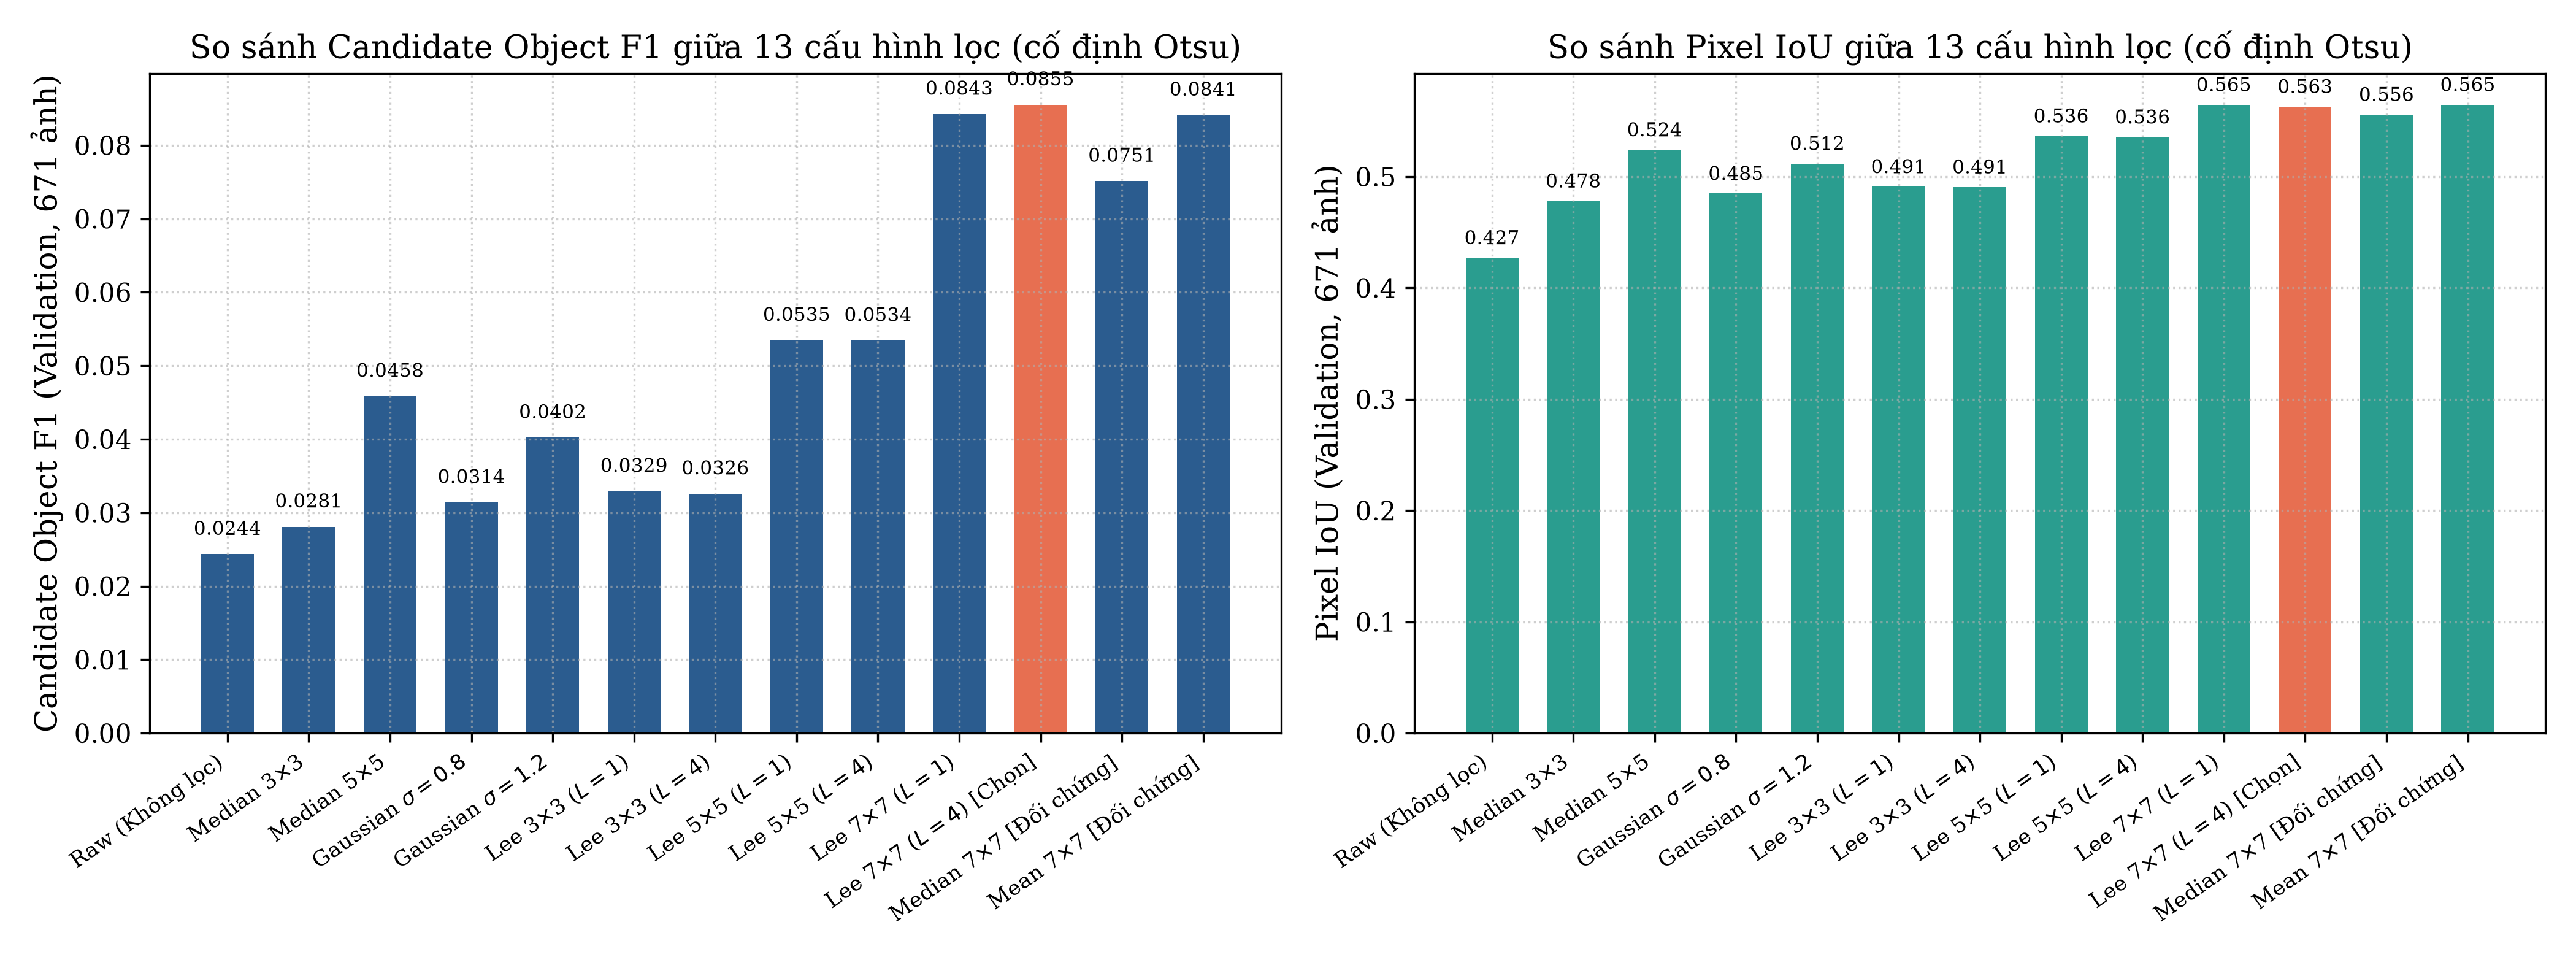
\includegraphics[width=\linewidth]{figures/fig4_filter_threshold_benchmark.png}
\caption{Đối sánh định lượng Candidate Object F1 và Pixel IoU giữa 13 cấu hình lọc không gian (cố định phân ngưỡng Otsu) trên toàn bộ 671 ảnh tập kiểm định (Validation).}
\label{fig:filter_benchmark}
\end{figure}

Kết quả thể hiện trong Bảng~\ref{tab:filter_benchmark}, Hình~\ref{fig:step_pipeline} và Hình~\ref{fig:filter_benchmark} đưa ra các phát hiện thực nghiệm quan trọng:
\begin{enumerate}
    \item \textbf{Hiệu quả giảm báo nhầm của kích thước cửa sổ lọc:} Trong lưới kích thước $\{3 \times 3, 5 \times 5, 7 \times 7\}$, việc mở rộng cửa sổ lọc lên biên trên $7 \times 7$ đóng vai trò quyết định trong việc giảm số lượng báo nhầm (từ $>46\,000$ FP xuống $\approx 20\,700$ FP, giảm hơn 55\% số mảnh nhiễu), đồng thời nâng Candidate F1 đơn điệu từ $0.0326$ ($3 \times 3$) lên $0.0534$ ($5 \times 5$) và đạt $0.0855$ ($7 \times 7$). Do $7 \times 7$ nằm tại biên trên của không gian tìm kiếm đã khóa, việc khảo sát các cửa sổ lớn hơn ($9 \times 9, 11 \times 11$) để xác định điểm uốn mà tại đó hiện tượng xóa nhòa dải dầu mảnh bắt đầu làm giảm Recall là hướng mở rộng cần thiết.
    \item \textbf{So sánh giữa Lee $7 \times 7$ và các bộ lọc đối chứng:} Trong không gian tìm kiếm ban đầu, cấu hình Lee $7 \times 7$ ($L=4$) đạt Candidate F1 cao nhất ($0.0855$). Tuy nhiên, phép đối chứng có kiểm soát bổ sung với cùng kích thước cửa sổ $7 \times 7$ cho thấy:
    \begin{itemize}
        \item Cấu hình Lee $7 \times 7$ ($L=1$, Candidate F1 $= 0.0843$) và bộ lọc trung bình Mean $7 \times 7$ (Candidate F1 $= 0.0841$) có hiệu năng tương đương thống kê với Lee $7 \times 7$ ($L=4$); độ lệch $\Delta\text{F1} = +0.0014$ so với Mean $7 \times 7$ có khoảng tin cậy Bootstrap 95\% $[-0.0003, +0.0033]$ chứa giá trị 0.
        \item Giải thích nguyên nhân: Như đã phân tích tại Mục~\ref{subsec:lee_filter}, do ảnh trong bộ dữ liệu SOS đã qua tiền xử lý đa nhìn và lượng tử hóa 8-bit ($[0, 1]$), hệ số biến thiên cục bộ $C_I^2(x, y) = v(x, y)/m^2(x, y)$ tại đại đa số các vùng biển và tâm vết dầu đều nhỏ hơn nhiều so với ngưỡng phương sai nhiễu giả định $1/L \in \{0.25, 1.0\}$. Hệ quả là $W(x, y) = \max(0, 1 - \frac{1/L}{C_I^2}) = 0$ trên toàn bộ vùng đồng nhất (như ở hàng 3 Hình~\ref{fig:step_pipeline} với $\max W = 0.00$) và chỉ kích hoạt nhẹ ($W > 0$) dọc theo ranh giới chuyển tiếp dốc. Do đó, bộ lọc Lee với $L \le 4$ trên ảnh PNG 8-bit thực chất hoạt động gần tương đương bộ lọc hộp Mean $7 \times 7$, và cả hai đều vượt trội có ý nghĩa thống kê so với Median $7 \times 7$ ($\Delta\text{F1} = +0.0104$, 95\% CI $[+0.0075, +0.0134]$).
    \end{itemize}
    \item \textbf{Nhánh phân ngưỡng cục bộ Niblack:} Khảo sát đầy đủ 9 cấu hình Niblack (kết hợp cùng bộ lọc Lee $7 \times 7, L=4$ tại $A_{\min} = 16$) trên tập kiểm định cho thấy hiệu năng suy giảm mạnh do hiện tượng bùng nổ báo nhầm ở vùng biển đồng nhất:
    \begin{itemize}
        \item Cửa sổ $15 \times 15$: $k=0.2 \to \text{F1}=0.0067$ ($\text{TP}=255, \text{FP}=75\,870$); $k=0.5 \to \text{F1}=0.0031$ ($\text{FP}=139\,556$); $k=0.8 \to \text{F1}=0.0013$ ($\text{FP}=154\,728$).
        \item Cửa sổ $31 \times 31$: $k=0.2 \to \text{F1}=0.0232$ ($\text{TP}=561, \text{FP}=46\,595$); $k=0.5 \to \text{F1}=0.0134$ ($\text{FP}=76\,925$); $k=0.8 \to \text{F1}=0.0083$ ($\text{FP}=89\,203$).
        \item Cửa sổ $51 \times 51$: $k=0.2 \to \text{F1}=0.0319$ ($\text{TP}=696, \text{FP}=40\,268, \text{IoU}=0.3144$); $k=0.5 \to \text{F1}=0.0241$ ($\text{FP}=59\,676$); $k=0.8 \to \text{F1}=0.0178$ ($\text{FP}=66\,610$).
    \end{itemize}
    Ngay cả cấu hình Niblack tốt nhất trên toàn bộ lưới 110 cấu hình (Lee $7 \times 7, L=1$ + Niblack $51 \times 51, k=0.2$) cũng chỉ đạt Candidate F1 $= 0.0325$, và sau khi ghép bộ phân loại học máy trên tập kiểm định chỉ đạt F1 $= 0.1447$ (CART) và $0.1380$ (LinearSVM). Ngưỡng cục bộ $T(x, y) = m_W - k s_W$ bị hạ thấp ở các vùng biển lặng gió tạo ra hàng chục nghìn mảnh tối vụn, do đó phân ngưỡng toàn cục Otsu là lựa chọn phù hợp hơn cho bước tạo ứng viên trên bộ dữ liệu này.
\end{enumerate}

\subsection{Phân tích đặc trưng, Khảo sát Ablation và Quá trình hội tụ SVM}
\label{subsec:feature_analysis}

\begin{figure*}[!t]
\centering
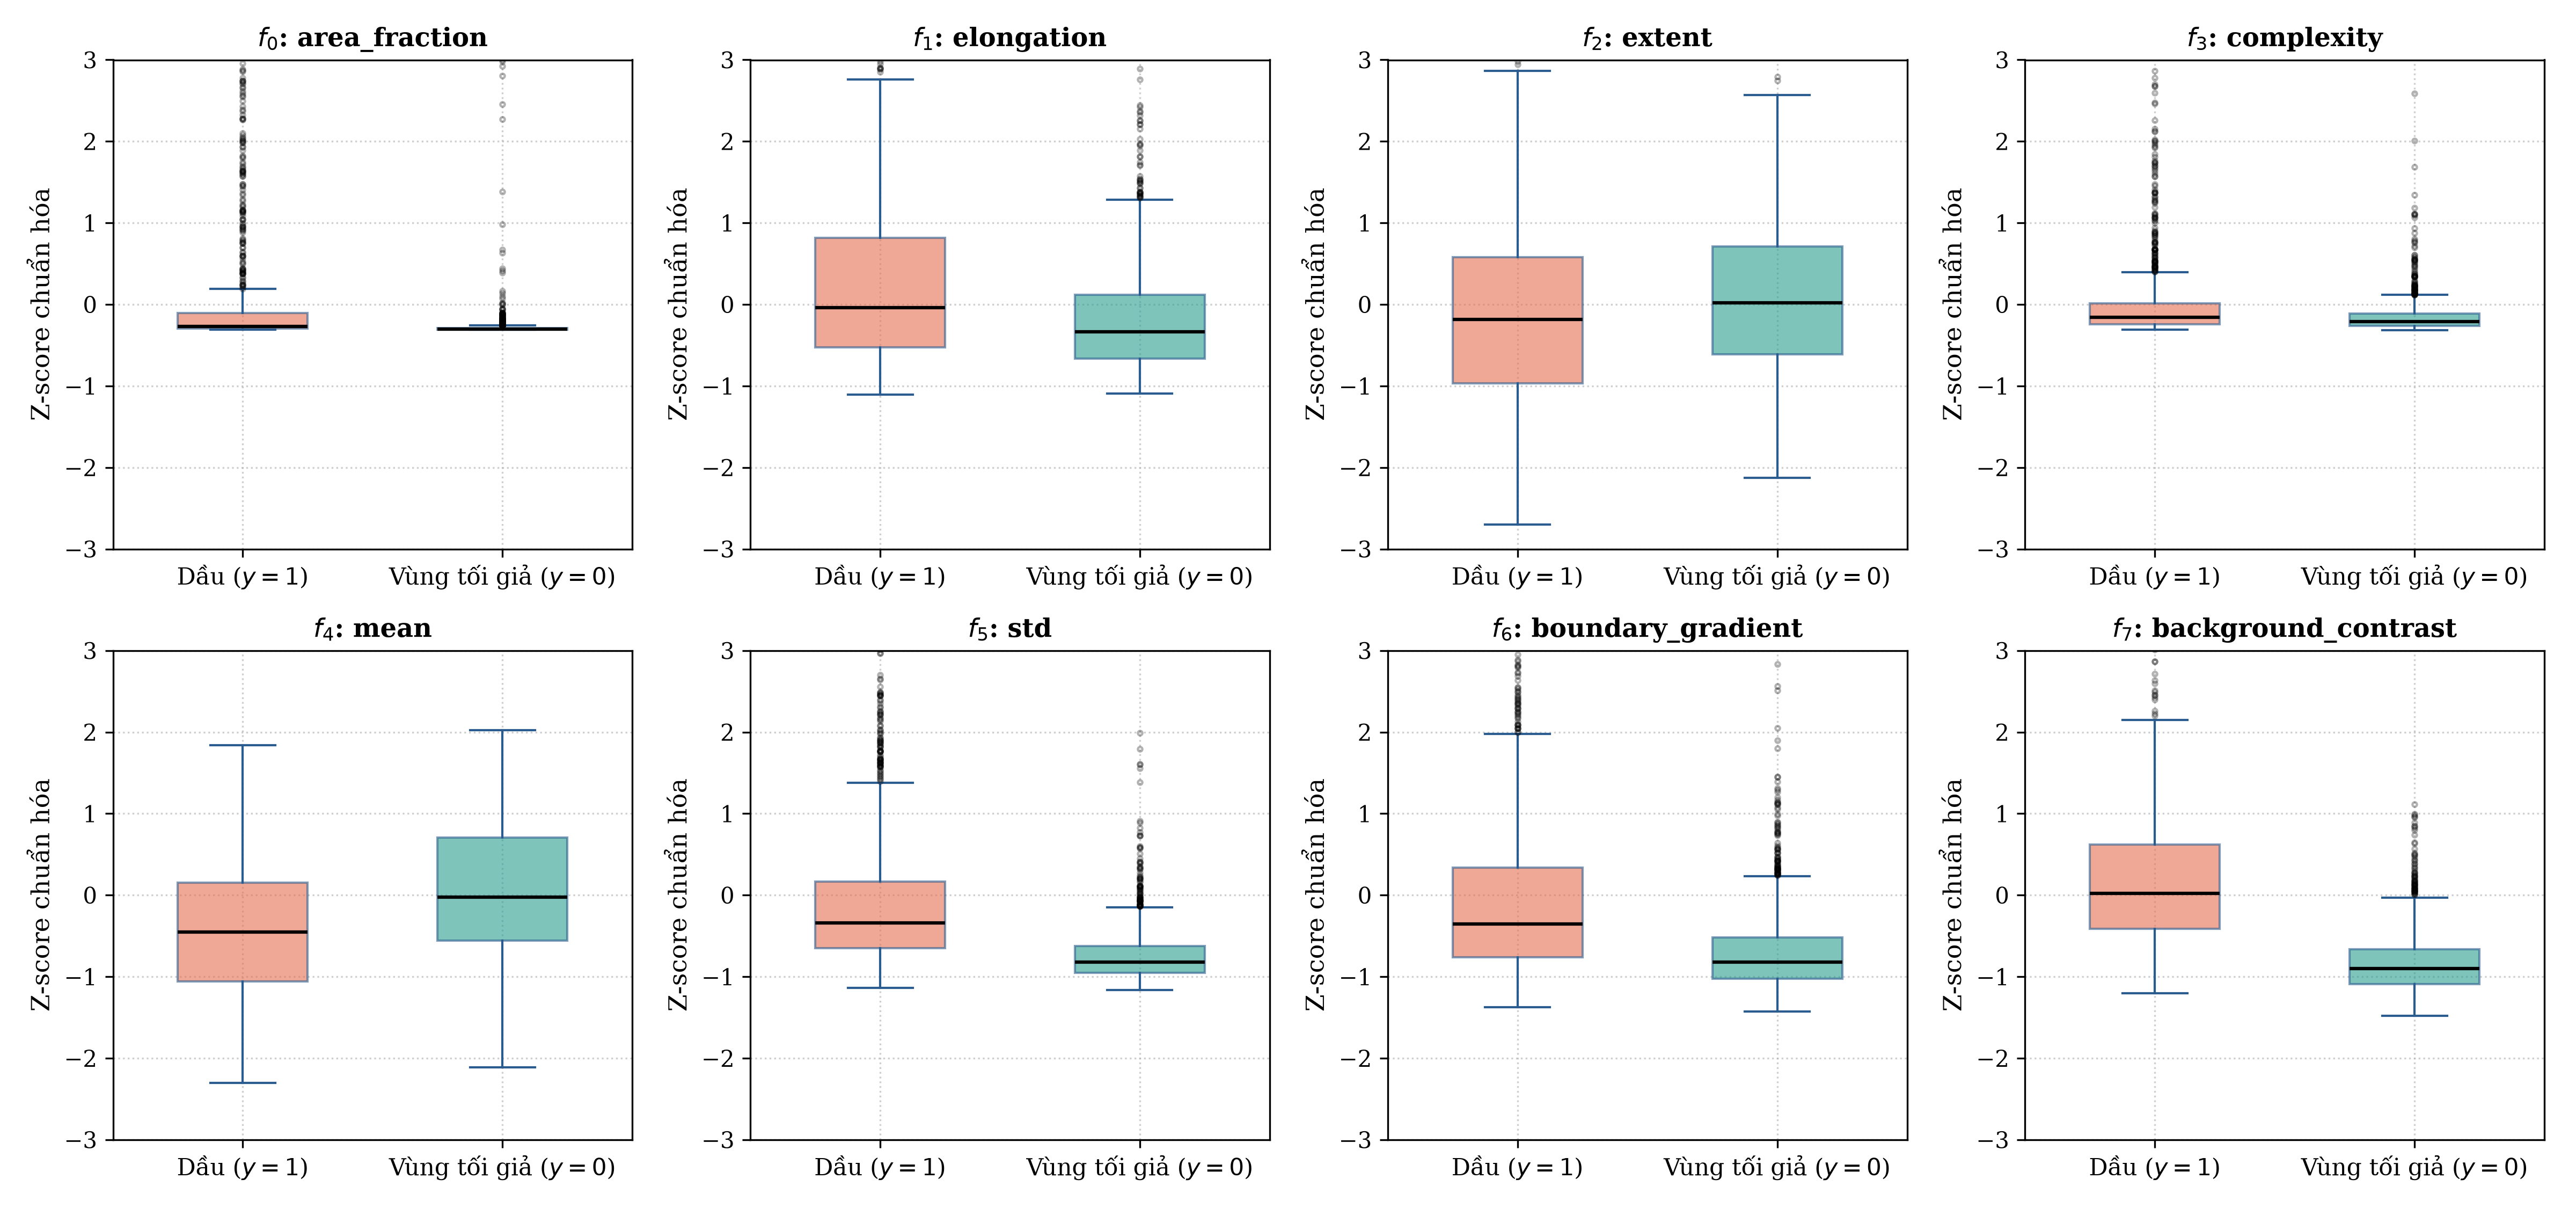
\includegraphics[width=0.95\textwidth]{figures/fig5_feature_distributions.png}
\caption{Biểu đồ Boxplot so sánh phân bố Z-score chuẩn hóa của 8 đặc trưng vùng giữa lớp Vết dầu thật ($\mathrm{Purity} \ge 0.50$, màu cam) và lớp Vùng tối báo nhầm ($\mathrm{Purity} \le 0.05$, màu xanh ngọc).}
\label{fig:feature_distributions}
\end{figure*}

\begin{figure}[!t]
\centering
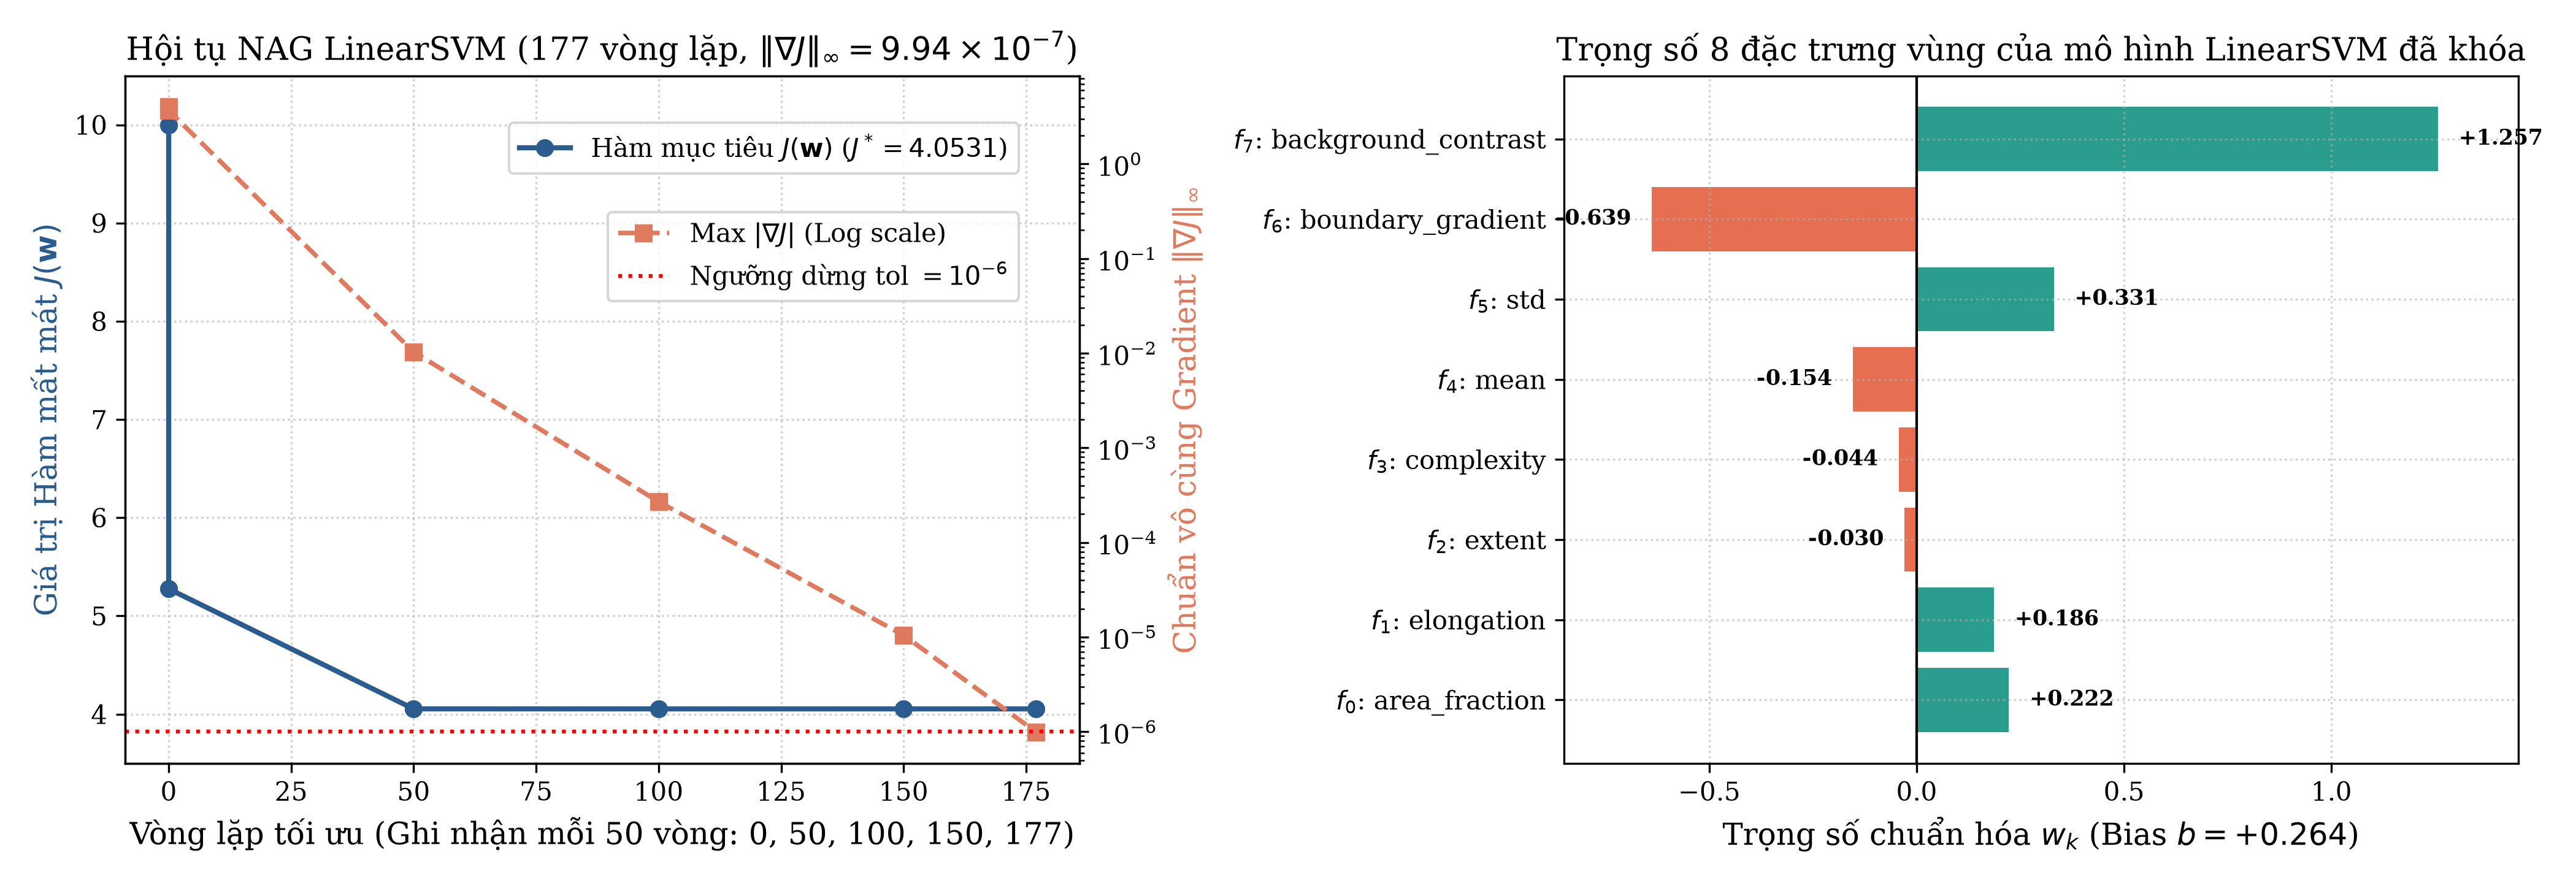
\includegraphics[width=\linewidth]{figures/fig6_svm_convergence_weights.png}
\caption{Đường cong hội tụ của thuật toán NAG ghi nhận tại các mốc 50 vòng lặp ($0, 50, 100, 150, 177$) cùng biểu đồ trọng số chuẩn hóa $w_k$ của 8 đặc trưng vùng trong mô hình LinearSVM đã khóa.}
\label{fig:svm_convergence}
\end{figure}

\begin{table}[!t]
\centering
\caption{Khảo sát hậu xử lý hình thái học, loại bỏ nhóm đặc trưng (Ablation study) và đối sánh mô hình trên tập kiểm định (671 ảnh Validation Sentinel-1A).}
\label{tab:ablation_validation}
\resizebox{\linewidth}{!}{%
\begin{tabular}{lccccc}
\toprule
\textbf{Cấu hình khảo sát} & \textbf{TP} & \textbf{FP} & \textbf{FN} & \textbf{Object F1} & \textbf{Pixel IoU} \\
\midrule
\multicolumn{6}{l}{\textit{Khảo sát ngưỡng diện tích $A_{\min}$ và hình thái học (Lee $7\times 7, L=4$ + Otsu + SVM):}} \\
$A_{\min} = 4$, \texttt{none} (Không đóng/mở) & $1\,035$ & $8\,571$ & $1\,705$ & 0.1677 & 0.6267 \\
$A_{\min} = 16$, \texttt{none} (Không đóng/mở) & $1\,034$ & $4\,482$ & $1\,706$ & 0.2505 & 0.6376 \\
$A_{\min} = 64$, \texttt{none} (\textbf{Chọn theo quy tắc}) & $\mathbf{1\,016}$ & $2\,215$ & $\mathbf{1\,724}$ & 0.3403 & \textbf{0.6524} \\
$A_{\min} = 64$, \texttt{close} (Đóng hình thái $3\times 3$) & 971 & $\mathbf{1\,961}$ & $1\,769$ & \textbf{0.3424} & 0.6402 \\
$A_{\min} = 64$, \texttt{open\_close} (Mở--Đóng $3\times 3$) & 988 & $2\,230$ & $1\,752$ & 0.3317 & 0.6505 \\
\midrule
\multicolumn{6}{l}{\textit{Ablation theo nhóm đặc trưng (LinearSVM, $C=10, A_{\min}=64$, \texttt{none}):}} \\
Chỉ đặc trưng hình học (\texttt{shape}, 4 chiều) & 736 & $1\,737$ & $2\,004$ & 0.2824 & 0.5899 \\
Chỉ đặc trưng bức xạ/biên (\texttt{intensity}, 4 chiều) & $1\,002$ & $2\,188$ & $1\,738$ & 0.3379 & \textbf{0.6542} \\
Kết hợp toàn bộ 8 đặc trưng (\texttt{all}, đề xuất) & $\mathbf{1\,016}$ & $2\,215$ & $\mathbf{1\,724}$ & \textbf{0.3403} & 0.6524 \\
\midrule
\multicolumn{6}{l}{\textit{So sánh bộ phân loại (Nhóm đặc trưng \texttt{all}, $A_{\min}=64$, \texttt{none}):}} \\
Cây quyết định CART ($\text{depth}=3, \text{leaf}=20$) & 961 & $\mathbf{1\,998}$ & $1\,779$ & 0.3373 & 0.6456 \\
LinearSVM ($C=10$, đề xuất) & $\mathbf{1\,016}$ & $2\,215$ & $\mathbf{1\,724}$ & \textbf{0.3403} & \textbf{0.6524} \\
\midrule
\multicolumn{6}{l}{\textit{Đánh giá cấp độ ứng viên theo nhãn Purity ($\mathrm{Purity} \ge 0.50$ vs.\ $\le 0.05$, $9\,287$ mẫu Val):}} \\
CART ($\text{TN}=6\,008$, Prec $=0.7952$, Rec $=0.7722$) & $2\,112$ & 544 & 623 & 0.7835 & -- \\
LinearSVM ($\text{TN}=5\,940$, Prec $=0.7874$, Rec $=0.8285$) & $\mathbf{2\,266}$ & 612 & $\mathbf{469}$ & \textbf{0.8074} & -- \\
\midrule
\multicolumn{6}{l}{\textit{Độ nhạy theo ngưỡng nhị phân Ground Truth (LinearSVM):}} \\
Ngưỡng mặt nạ GT $M_{\text{raw}} \ge 64$ & $1\,027$ & $2\,204$ & $1\,690$ & 0.3453 & 0.6526 \\
Ngưỡng mặt nạ GT $M_{\text{raw}} \ge 128$ (Chuẩn) & $1\,016$ & $2\,215$ & $1\,724$ & 0.3403 & 0.6524 \\
Ngưỡng mặt nạ GT $M_{\text{raw}} \ge 192$ & $1\,010$ & $2\,221$ & $1\,752$ & 0.3371 & 0.6517 \\
\bottomrule
\end{tabular}%
}
\end{table}

Hình~\ref{fig:feature_distributions} biểu diễn phân bố Z-score của 8 đặc trưng vùng giữa hai lớp, và Hình~\ref{fig:svm_convergence} thể hiện đường cong hội tụ cùng trọng số của mô hình LinearSVM đã khóa. Các kết quả mang lại các quan sát định lượng rõ ràng:
\begin{itemize}
    \item \textbf{Trọng số và cơ chế phân loại của LinearSVM:} Trong vector trọng số chuẩn hóa 9 chiều ($\mathbf{w} \in \mathbb{R}^8$ và hệ số chặn $b = +0.264$), trọng số dương lớn nhất thuộc về \texttt{background\_contrast} ($w_7 = +1.257$), theo sau bởi \texttt{std} ($w_5 = +0.331$), \texttt{area\_fraction} ($w_0 = +0.222$) và \texttt{elongation} ($w_1 = +0.186$). Ngược lại, trọng số âm lớn nhất rơi vào \texttt{boundary\_gradient} ($w_6 = -0.639$) và \texttt{mean} ($w_4 = -0.154$), trong khi \texttt{complexity} ($w_3 = -0.044$) và \texttt{extent} ($w_2 = -0.030$) nhận trọng số âm nhỏ.
    \item \textbf{Giải thích hiện tượng đa cộng tuyến và biến ức chế (Suppressor Variable) tại $w_6 = -0.639$:} Quan sát Hình~\ref{fig:feature_distributions} cho thấy xét đơn biến (univariate), các vùng dầu thật ($y=1$) thực tế có trung vị \texttt{boundary\_gradient} ($f_6$) cao hơn vùng tối giả ($y=0$), với hệ số tương quan điểm--nhị phân dương $\mathrm{Corr}(f_6, y) = +0.3632$ (cùng chiều với $\mathrm{Corr}(f_7, y) = +0.6485$, $\mathrm{Corr}(f_5, y) = +0.4499$ và ngược chiều với $\mathrm{Corr}(f_4, y) = -0.3413$). Tuy nhiên, trong mô hình tuyến tính đa biến, $f_6$ lại mang trọng số âm lớn $w_6 = -0.639$. Phân tích ma trận tương quan trên tập huấn luyện làm sáng tỏ nguyên nhân: \texttt{boundary\_gradient} có tương quan dương rất mạnh với cả độ lệch chuẩn nội vùng $\mathrm{Corr}(f_6, f_5) = +0.8504$ lẫn độ tương phản nền $\mathrm{Corr}(f_6, f_7) = +0.6716$. Khi tổ hợp tuyến tính đã gán trọng số dương rất lớn cho $w_7 = +1.257$ và $w_5 = +0.331$, đặc trưng $f_6$ đóng vai trò là một \textit{biến ức chế (suppressor variable)} cổ điển: trọng số âm $w_6 = -0.639$ giúp hiệu chỉnh phần phương sai dư thừa của các vùng có đạo hàm biên gắt nhân tạo do cắt ngưỡng hoặc nhiễu cục bộ ($f_6$ lớn, $f_5$ lớn) nhưng không đi kèm độ chênh lệch tương phản nền tương xứng ($f_7$).
    \item \textbf{Khảo sát hình thái học, ngưỡng diện tích và Ablation (Bảng~\ref{tab:ablation_validation}):}
    \begin{enumerate}
        \item \textit{Tác động của $A_{\min}$ và phép đóng/mở hình thái:} Việc nâng ngưỡng diện tích tối thiểu từ $A_{\min} = 4$ lên $16$ và $64$ pixels giúp cắt giảm mạnh số lượng mảnh nhiễu (từ $8\,571$ xuống $4\,482$ và $2\,215$ FP) trong khi hầu như không làm giảm số lượng đối tượng đúng ($\text{TP}$ chỉ giảm nhẹ từ $1\,035$ xuống $1\,016$), qua đó nâng Object F1 từ $0.1677$ lên $0.3403$. Tại mức $A_{\min} = 64$, phép đóng hình thái \texttt{close} đạt Object F1 cao hơn nhẹ ($0.3424$ so với $0.3403$ của \texttt{none}), nhưng vì chênh lệch này nằm trong dải dung sai lựa chọn $\Delta\text{F1} \le 0.005$ đã định nghĩa trước ở Mục~\ref{subsec:dataset}, quy tắc ưu tiên độ thu hồi Recall cao hơn ($0.3708$ với $1\,016$ TP của \texttt{none} so với $0.3544$ với $971$ TP của \texttt{close}) đã chọn cấu hình \texttt{none} để tránh làm dính liền các vệt dầu lân cận.
        \item \textit{Đóng góp của các nhóm đặc trưng:} Nhóm đặc trưng bức xạ/biên (\texttt{intensity}, 4 chiều) giữ vai trò quyết định với Object F1 $= 0.3379$ và Pixel IoU $= 0.6542$, vượt xa nhóm đặc trưng hình học thuần túy (\texttt{shape}, F1 $= 0.2824$). Việc bổ sung 4 đặc trưng hình học vào nhóm bức xạ (\texttt{all}, 8 chiều) mang lại mức cải thiện khiêm tốn ($+0.0024$ Object F1, từ $0.3379$ lên $0.3403$), khẳng định thông tin bức xạ đóng vai trò chủ đạo trên bộ dữ liệu này.
        \item \textit{So sánh LinearSVM và CART:} Trên thước đo đối tượng Hungarian ($\IoU \ge 0.50$), hai mô hình có hiệu năng sát nhau (LinearSVM đạt F1 $= 0.3403$, Recall $= 0.3708$; CART đạt F1 $= 0.3373$, Precision cao hơn ở mức $0.3248$). Xét riêng ở cấp độ phân loại từng ứng viên theo nhãn Purity ($\mathrm{Purity} \ge 0.50$ so với $\le 0.05$ trên $9\,287$ mẫu kiểm định rõ nghĩa), LinearSVM đạt F1 cấp ứng viên $80.74\%$ ($\text{TP}=2\,266, \text{FP}=612, \text{TN}=5\,940, \text{FN}=469$), nhỉnh hơn CART ($78.35\%$, $\text{TP}=2\,112, \text{FP}=544, \text{TN}=6\,008, \text{FN}=623$) nhờ giữ lại nhiều hơn $154$ vùng dầu thật. Cả hai bản tự cài bằng NumPy đều đạt độ đồng thuận dự đoán 100\% so với triển khai tham chiếu \texttt{scikit-learn}.
    \end{enumerate}
    \item \textbf{Quá trình hội tụ NAG:} Thuật toán NAG hội tụ sau 177 vòng lặp (Hình~\ref{fig:svm_convergence} vẽ theo chu kỳ ghi nhật ký mỗi 50 vòng lặp tại các mốc $0, 50, 100, 150$ và điểm dừng $177$), đưa hàm mục tiêu từ $J(\mathbf{0}) = 10.0$ xuống $J^* = 4.0531$ và đạt chuẩn vô cùng gradient $\|\nabla J\|_\infty = 9.94 \times 10^{-7} \le 10^{-6}$.
\end{itemize}

\subsection{Đánh giá so sánh định lượng và định tính trên tập kiểm thử độc lập}
\label{subsec:quantitative_eval}

\begin{table*}[!t]
\centering
\caption{Đánh giá so sánh hiệu năng trên tập kiểm thử độc lập (839 ảnh Sentinel-1A và 776 ảnh ALOS PALSAR). Giao thức ghép cặp đối tượng Hungarian ở ngưỡng $\IoU \ge 0.5$. Khoảng tin cậy Bootstrap 95\% trên tập Sentinel-1A: Object F1 đạt $0.2805 \ [0.2652, 0.2980]$ (LinearSVM) so với $0.1220 \ [0.1124, 0.1328]$ (Không Classifier), mức tăng $\Delta\text{F1} = +0.1586 \ [+0.1474, +0.1706]$.}
\label{tab:model_comparison}
\resizebox{\textwidth}{!}{%
\begin{tabular}{lcccccccccc}
\toprule
\textbf{Phương pháp} & \textbf{Ảnh} & \textbf{TP} & \textbf{FP} & \textbf{FN} & \textbf{Prec} & \textbf{Rec} & \textbf{Obj F1} & \textbf{Pix IoU} & \textbf{FP/ảnh} & \textbf{Edge / Int Rec} \\
\midrule
\textit{Baseline (Ảnh thô + Otsu, $A_{\min} = 16$)} & 839 & 426 & $49\,182$ & $2\,756$ & 0.0086 & 0.1339 & 0.0161 & 0.4367 & 58.62 & 0.1979 / 0.0038 \\
\textit{Lee 7$\times$7 + Otsu ($A_{\min} = 64$, Không Clf)} & 839 & $1\,018$ & $12\,495$ & $2\,164$ & 0.0753 & \textbf{0.3199} & 0.1220 & 0.5867 & 14.89 & \textbf{0.4221} / \textbf{0.1124} \\
\textbf{Pipeline + LinearSVM ($A_{\min} = 64$, Đề xuất)} & 839 & 996 & $\mathbf{2\,923}$ & $2\,186$ & \textbf{0.2541} & 0.3130 & \textbf{0.2805} & \textbf{0.6614} & \textbf{3.48} & 0.4156 / 0.1048 \\
\quad \textit{Macro từng ảnh ($\text{mean} \pm \text{SD}$)$^{\dagger}$} & \multicolumn{4}{c}{--} & $0.356 \pm 0.336$ & $0.446 \pm 0.382$ & $0.349 \pm 0.317$ & $0.577 \pm 0.261$ & $3.48 \pm 3.97$ & -- \\
\midrule
\textit{Ngoài cảm biến: PALSAR (LinearSVM, $A_{\min} = 64$)} & 776 & $1\,441$ & $2\,305$ & $2\,553$ & 0.3847 & 0.3608 & 0.3724 & 0.6423 & 2.97 & 0.4587 / 0.1890 \\
\quad \textit{Macro từng ảnh ($\text{mean} \pm \text{SD}$)$^{\ddagger}$} & \multicolumn{4}{c}{--} & $0.465 \pm 0.342$ & $0.438 \pm 0.338$ & $0.412 \pm 0.312$ & $0.579 \pm 0.234$ & $2.97 \pm 3.43$ & -- \\
\bottomrule
\multicolumn{11}{l}{\footnotesize $^{\dagger}$Cỡ mẫu mẫu số khác không trên Sentinel-1A (839 ảnh): $n_{\text{Prec}}=786$, $n_{\text{Rec}}=808$, $n_{\text{F1}}=n_{\text{IoU}}=814$ ($25$ ảnh $R_0$ có $\text{TP}=\text{FP}=\text{FN}=0$).} \\
\multicolumn{11}{l}{\footnotesize $^{\ddagger}$Cỡ mẫu mẫu số khác không trên ALOS PALSAR (776 ảnh): $n_{\text{Prec}}=705$, $n_{\text{Rec}}=731$, $n_{\text{F1}}=n_{\text{IoU}}=734$ ($42$ ảnh $R_0$ có $\text{TP}=\text{FP}=\text{FN}=0$).}
\end{tabular}%
}
\end{table*}

\begin{figure*}[!t]
\centering
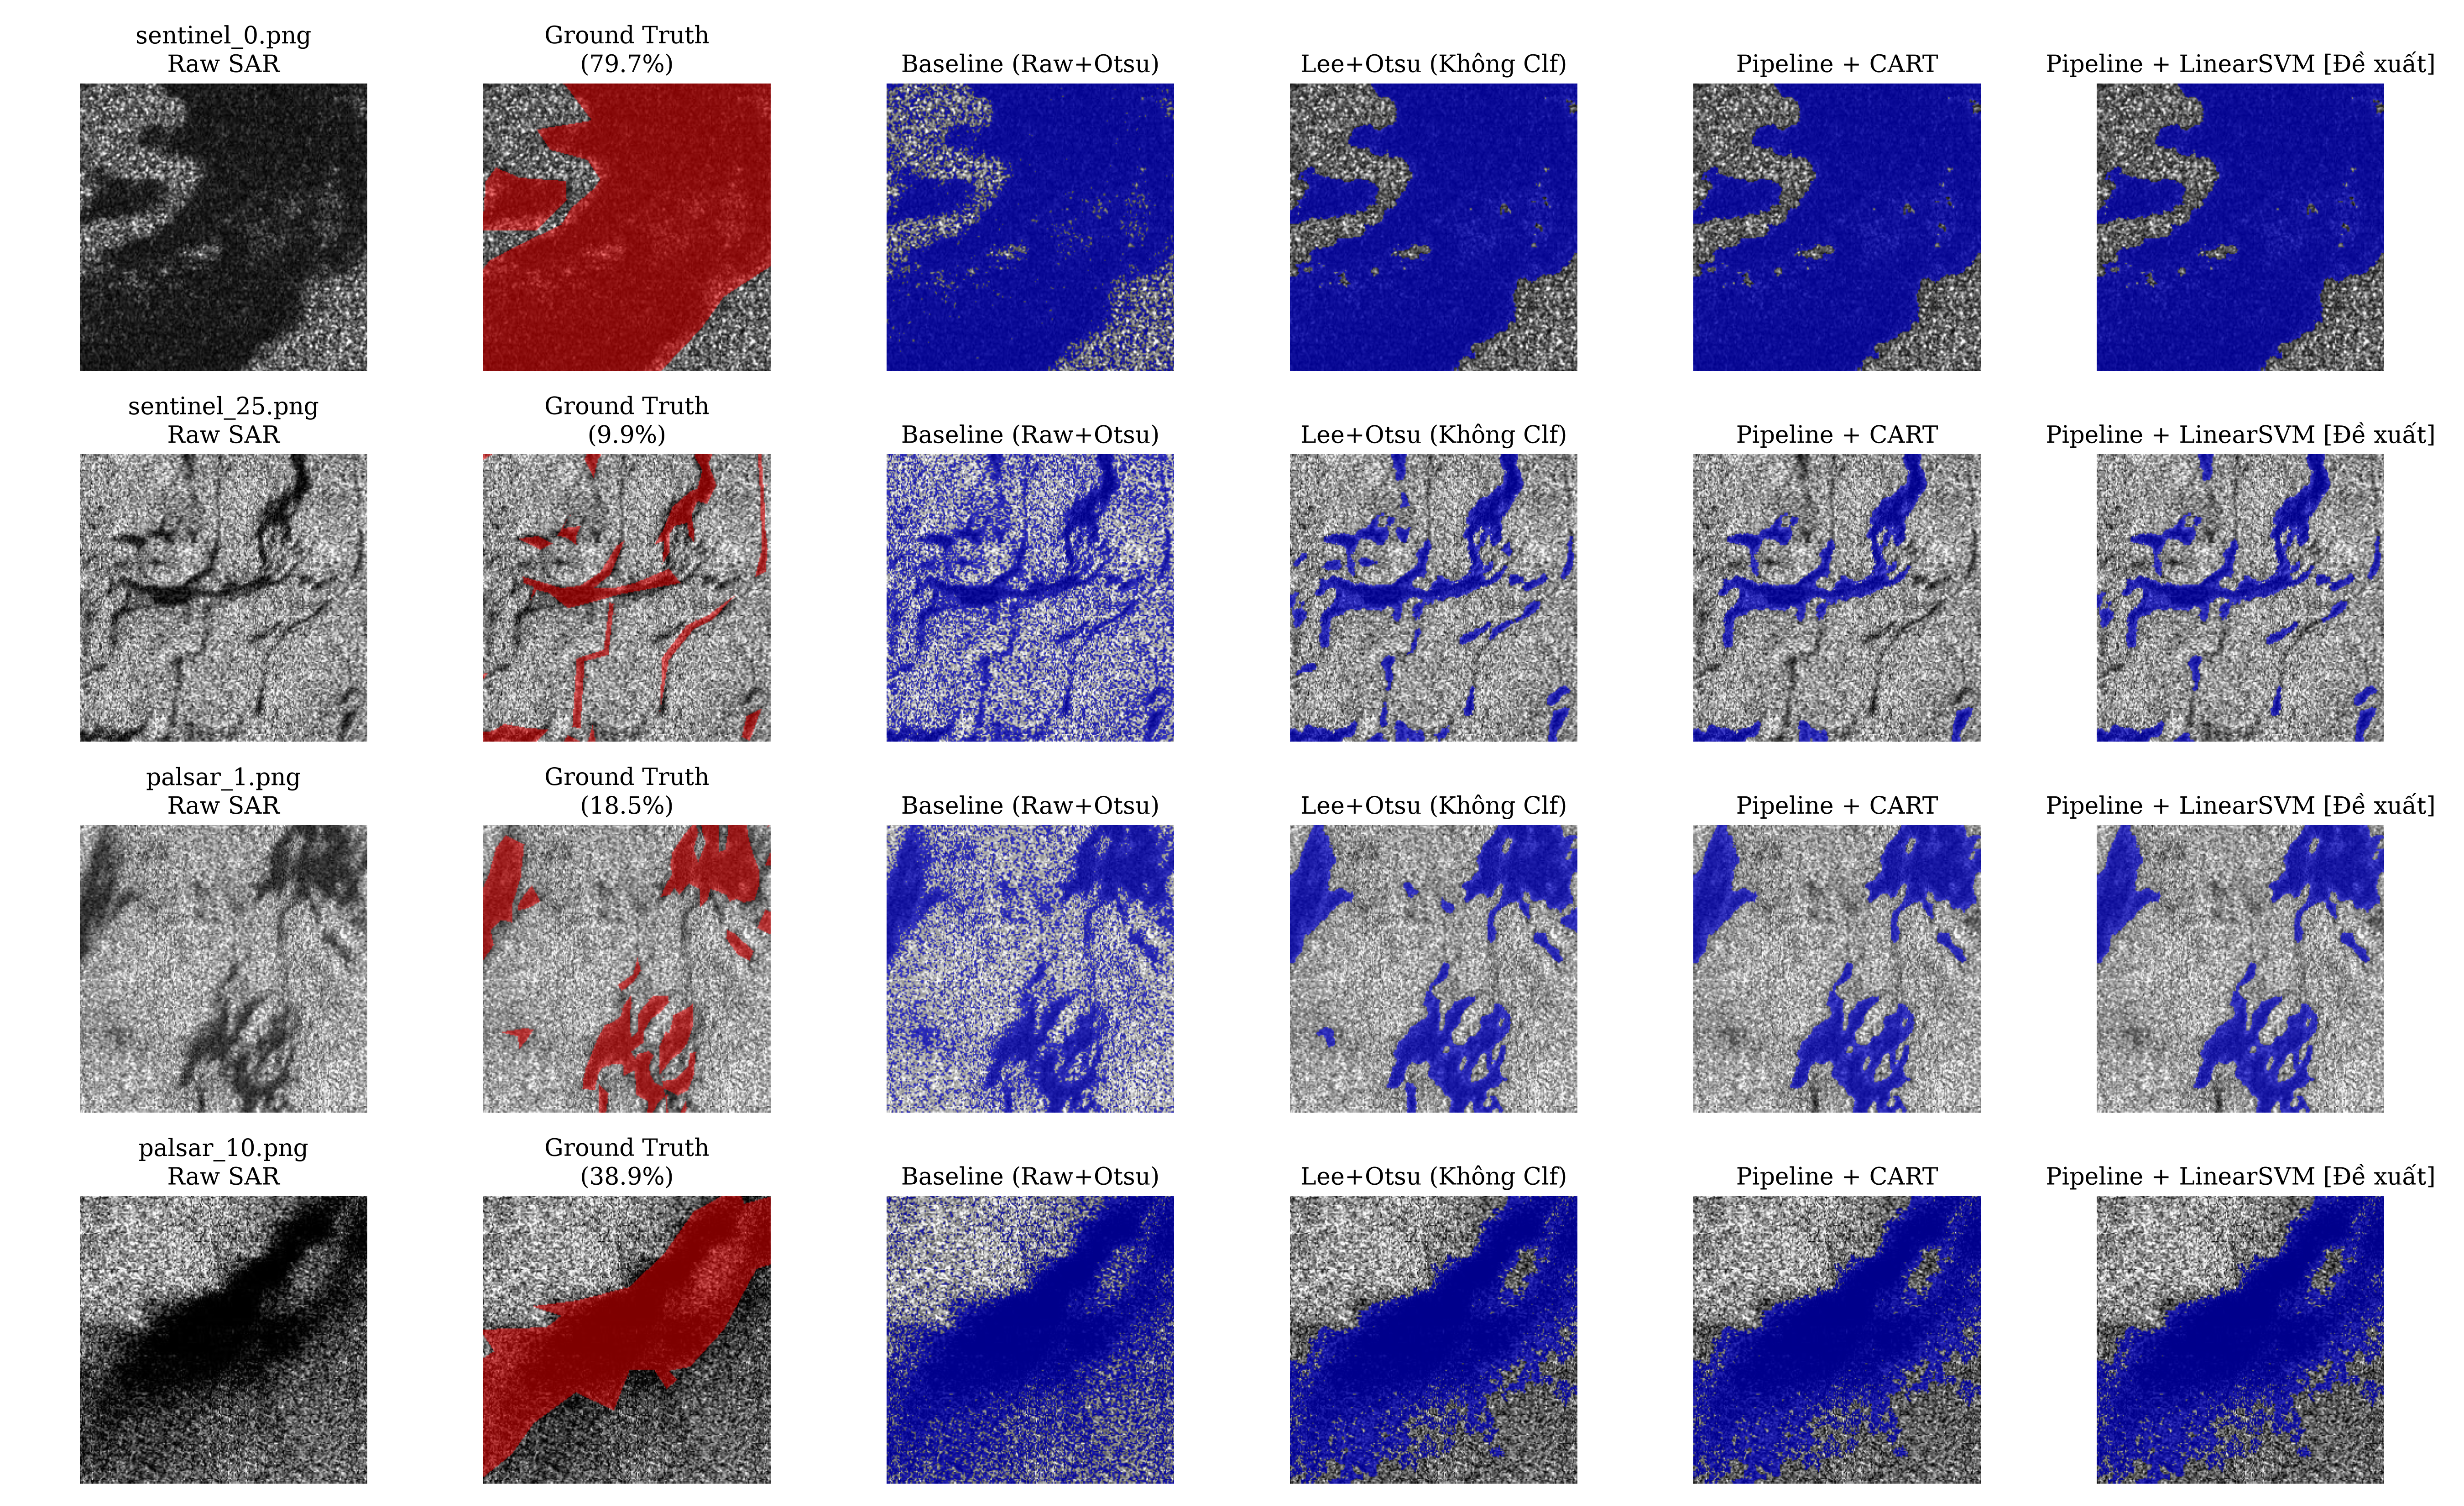
\includegraphics[width=\textwidth]{figures/fig7_qualitative_comparison.png}
\caption{Đối sánh định tính kết quả phân đoạn giữa các mô hình trên 4 cảnh SAR điển hình (\texttt{val/sentinel\_0.png}, \texttt{val/sentinel\_25.png}, \texttt{val/palsar\_1.png}, \texttt{val/palsar\_10.png}): Cột 1: Ảnh thô; Cột 2: Mặt nạ Ground Truth; Cột 3: Baseline (Ảnh thô + Otsu, $A_{\min}=16$); Cột 4: Lọc Lee + Otsu ($A_{\min}=64$, Không classifier); Cột 5: Pipeline + CART; Cột 6: Pipeline + LinearSVM (Đề xuất).}
\label{fig:qualitative_comparison}
\end{figure*}

Bảng~\ref{tab:model_comparison} tổng hợp kết quả đánh giá thực nghiệm định lượng trên tập kiểm thử độc lập ($839$ ảnh Sentinel-1A, chứa tổng cộng $3\,182$ đối tượng dầu Ground Truth). Các số liệu thực nghiệm làm rõ đóng góp của từng thành phần cũng như các giới hạn cấu trúc của phương pháp:
\begin{itemize}
    \item \textbf{Bóc tách hiệu quả của Giai đoạn 1 và Giai đoạn 2:}
    \begin{enumerate}
        \item \textit{Từ Baseline thô sang Giai đoạn 1 (Lọc Lee $7 \times 7$ + Otsu + $A_{\min} = 64$):} Tỷ lệ báo nhầm giảm từ $58.62$ xuống $14.89$ FP/ảnh (tổng số ứng viên giảm từ $49\,608$ xuống $13\,513$), đồng thời số đối tượng dầu phát hiện đúng tăng từ $426$ lên $1\,018$ TP. Lưu ý rằng bước nhảy này là kết quả tổng hợp của hai yếu tố: bộ lọc Lee $7 \times 7$ làm mượt nhiễu đốm (giúp giảm $\approx 47\%$ số FP ở cùng ngưỡng $A_{\min} = 16$, như đã chứng minh có kiểm soát tại Bảng~\ref{tab:filter_benchmark}) và việc nâng ngưỡng cắt tỉa diện tích từ $A_{\min} = 16$ (của Baseline mặc định) lên $A_{\min} = 64$ (giúp loại bỏ tiếp hơn một nửa số mảnh nhiễu nhỏ còn lại, như đã bóc tách tại Bảng~\ref{tab:ablation_validation}).
        \item \textit{Từ Giai đoạn 1 sang Giai đoạn 2 (Bổ sung bộ phân loại LinearSVM ở cùng $A_{\min} = 64$):} Đây là phép so sánh có kiểm soát hoàn toàn cho riêng bộ phân loại vùng. So với cấu hình \textit{Không dùng Classifier} ($\text{TP}=1\,018, \text{FP}=12\,495$), LinearSVM đã \textbf{loại bỏ được $9\,572$ vùng báo nhầm} (giảm $76.6\%$ FP/ảnh, từ $14.89$ xuống $3.48$ FP/ảnh), trong khi \textbf{giữ lại được $97.8\%$ số đối tượng đúng của giai đoạn tạo ứng viên} ($996 / 1\,018$ TP, chỉ mất 22 vùng và đạt độ thu hồi tổng thể $\text{Recall} = 0.3130$ trên tổng số $3\,182$ đối tượng GT toàn tập). Nhờ đó, Precision tăng $3.37$ lần (từ $0.0753$ lên $0.2541$), Object F1 tăng từ $0.1220$ lên $0.2805$ ($\Delta\text{F1} = +0.1586$, 95\% CI $[+0.1474, +0.1706]$) và Pixel IoU toàn cục tăng từ $0.5867$ lên $0.6614$.
    \end{enumerate}
    \item \textbf{Giải phẫu sự vênh giữa độ chính xác phân loại Purity và chỉ số Object F1:} Một câu hỏi quan trọng là vì sao LinearSVM đạt F1 cấp độ ứng viên tới $80.74\%$ theo nhãn Purity nhưng Object F1 cuối cùng chỉ đạt $0.3403$ (Validation) và $0.2805$ (Test). Đối chiếu ma trận nhầm lẫn cấp ứng viên trên tập Validation (Bảng~\ref{tab:ablation_validation}) với kết quả ghép cặp Hungarian ($\text{TP}_{\text{IoU}} = 1\,016, \text{FP}_{\text{IoU}} = 2\,215$) cho thấy: trong số $2\,878$ vùng được LinearSVM dự đoán là dầu ($\hat{y}_i = 1$ trên các mẫu rõ nghĩa), chỉ có \textbf{$612$ vùng ($21.3\%$) là báo nhầm nền biển thực sự} ($\mathrm{Purity} \le 0.05$). Ngược lại, có tới \textbf{$2\,266$ vùng dự đoán dương tính thực sự nằm đè lên vết dầu thật} ($\mathrm{Purity} \ge 0.50$), nhưng chỉ có $1\,016$ vùng trong số đó vượt qua ngưỡng ghép cặp 1--1 $\IoU \ge 0.50$ để trở thành $\text{TP}_{\text{IoU}}$; hơn \textbf{$1\,250$ mảnh dầu thật còn lại bị giao thức Hungarian xếp vào nhóm $\text{FP}_{\text{IoU}}$} (chiếm tới $56.4\%$ tổng số $2\,215$ FP đối tượng!). Nói cách khác, phần lớn ``False Positives'' ở cấp độ đối tượng không phải do bộ phân loại nhận nhầm nước biển thành dầu, mà là hệ quả của việc một vết dầu lớn bị Otsu cắt rời thành nhiều mảnh con có $\mathrm{Purity} \ge 0.50$ nhưng mỗi mảnh có $\IoU < 0.50$ so với mặt nạ GT nguyên khối.
    \item \textbf{Nút cổ chai độ thu hồi (Recall Bottleneck Analysis):} Bảng~\ref{tab:model_comparison} chỉ rõ rằng Recall sau phân loại ($0.3130$) bị khống chế trực tiếp bởi trần Recall của giai đoạn 1 ($0.3199$). Do bộ phân loại vùng chỉ thực hiện lọc bỏ ứng viên chứ không thể khôi phục các vùng bị bỏ sót, Recall của hệ thống bị giới hạn bởi bước phân đoạn toàn cục Otsu. Đáng chú ý, phân tích theo vị trí đối tượng cho thấy thuật toán đạt Recall tương đối tốt trên các vết dầu lớn chạm biên khung ảnh (\texttt{Edge Recall} $= 41.56\%$), nhưng gặp khó khăn lớn đối với các vệt dầu nhỏ nằm trọn bên trong khung ảnh (\texttt{Interior Recall} chỉ đạt $10.48\%$).
    \item \textbf{Phân tích hậu nghiệm ba cơ chế lỗi điển hình (Post-hoc Error Diagnostics):} Để minh họa trực quan các giới hạn vật lý của quy trình, chúng tôi trích xuất hậu nghiệm 3 trường hợp thất bại cực đoan nhất từ tập kiểm thử (\texttt{val/}) sau khi đã khóa hoàn toàn mô hình (không sử dụng cho bất kỳ quyết định lựa chọn tham số nào):
    \begin{enumerate}
        \item \textit{Phân mảnh vệt dầu lớn thành nhiều FP đối tượng} (Ảnh \texttt{val/sentinel\_440.png}, chế độ $R_4$ ngập 100\% dầu): Do histogram đơn đỉnh, Otsu cắt đôi mảng dầu thành 35 mảnh ứng viên nhỏ. Dù toàn bộ 35 mảnh này đều có $\mathrm{Purity} = 1.00$ (nằm trọn trên dầu thật), không mảnh nào đủ lớn để đạt $\IoU \ge 0.5$ với mặt nạ GT nguyên khối duy nhất, dẫn đến hệ thống bị phạt đồng thời $0$ TP, $35$ FP và $1$ FN.
        \item \textit{Bỏ sót dải dầu mảnh} (Ảnh \texttt{val/sentinel\_25.png}, chế độ $R_2$): Các vệt dầu hẹp có độ tương phản yếu bị ngưỡng Otsu toàn cục nâng quá cao bỏ sót ngay từ Giai đoạn 1, gây ra $20$ FN.
        \item \textit{Suy biến vành đai nền ở vùng ngập dầu} (Ảnh \texttt{val/sentinel\_591.png}, chế độ $R_3$): Bước phân ngưỡng ban đầu làm mất hơn $38\,000$ điểm ảnh dầu, và bộ phân loại tiếp tục loại bỏ các vùng còn lại do vành đai nền bị ép vào các điểm ảnh rìa sáng vượt ngưỡng Otsu, làm sai lệch hoàn toàn đặc trưng tương phản nền.
    \end{enumerate}
    \item \textbf{Hiệu năng tính toán:} Toàn bộ pipeline cài đặt bằng NumPy thuần chạy trên CPU (đo lường qua thực thi song song 4 tiến trình worker trên 839 ảnh Test) đạt thời gian thông lượng trung bình $50.2 \pm 14.7\text{ ms/ảnh}$ (tổng thời gian $42.11$ giây), nhanh hơn gấp đôi so với cấu hình Baseline thô ($90.46$ giây, $107.8\text{ ms/ảnh}$). Nguyên nhân giúp pipeline đầy đủ chạy nhanh hơn cấu hình không lọc là do bước lọc Lee $7 \times 7$ kết hợp $A_{\min} = 64$ đã thu gọn số lượng thành phần liên thông cần duyệt và trích xuất đặc trưng xuống chỉ còn $13\,513$ vùng (so với $49\,608$ vùng nhiễu vụn ở Baseline thô).
\end{itemize}

\subsection{Hiệu năng phân tầng theo 5 chế độ diện tích và Đánh giá ngoài cảm biến}
\label{subsec:regime_analysis}

\begin{figure}[!t]
\centering
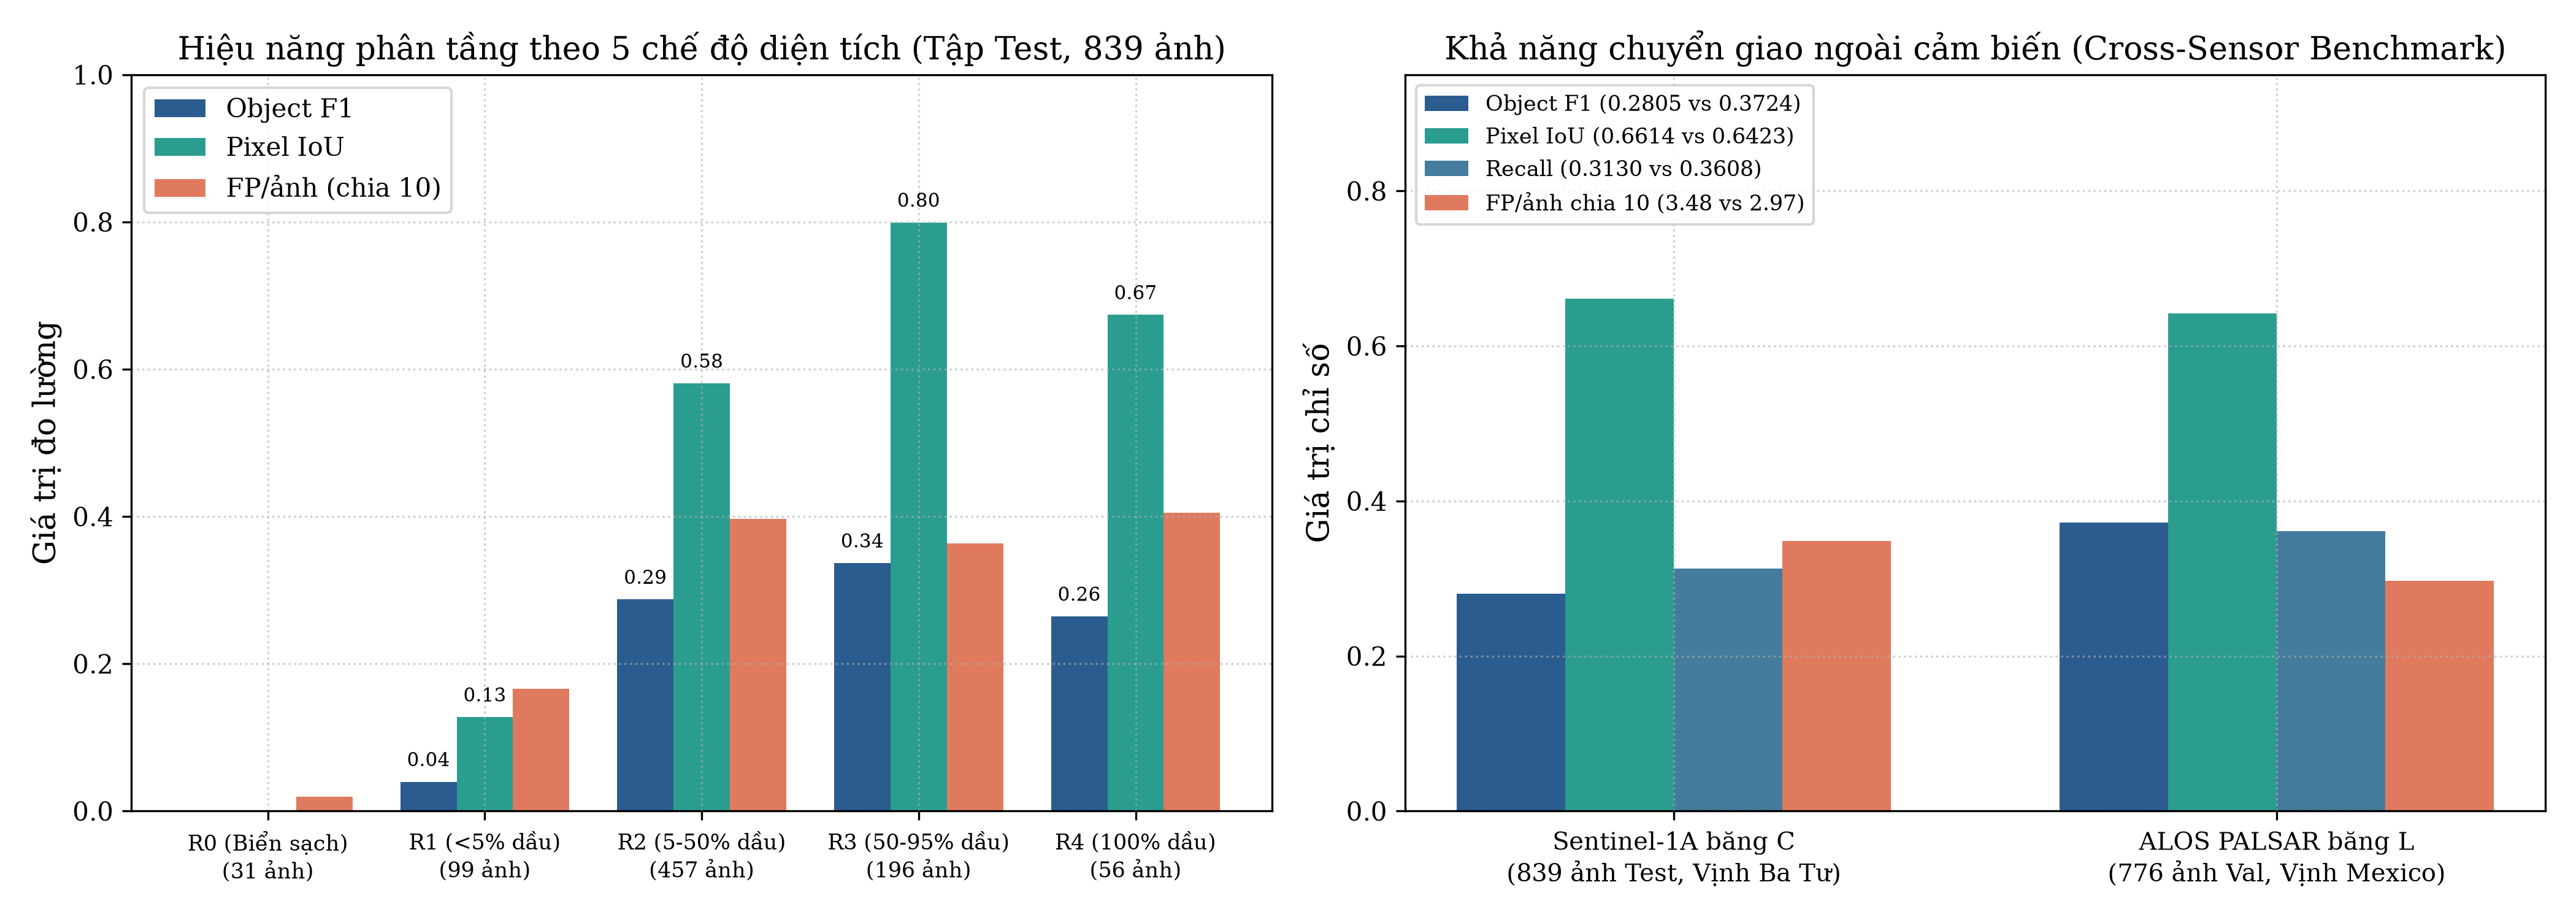
\includegraphics[width=\linewidth]{figures/fig8_regime_sensor_performance.png}
\caption{Hiệu năng phân tầng của mô hình đề xuất theo 5 chế độ diện tích dầu ($R_0 \to R_4$, bên trái) trên 839 ảnh Test Sentinel-1A và đối sánh khả năng chuyển giao ngoài cảm biến sang 776 ảnh ALOS PALSAR (bên phải).}
\label{fig:regime_sensor}
\end{figure}

\begin{table}[!t]
\centering
\caption{Chi tiết hiệu năng phân tầng của mô hình đề xuất (LinearSVM) theo 5 chế độ diện tích dầu ($R_0 \to R_4$) trên cả hai tập kiểm thử độc lập: 839 ảnh Sentinel-1A (băng C) và 776 ảnh ALOS PALSAR (băng L).}
\label{tab:regime_breakdown}
\resizebox{\linewidth}{!}{%
\begin{tabular}{lccccccc}
\toprule
\textbf{Chế độ diện tích} & \textbf{Số ảnh} & \textbf{TP} & \textbf{FP} & \textbf{FN} & \textbf{Object F1} & \textbf{Pixel IoU} & \textbf{FP / ảnh} \\
\midrule
\multicolumn{8}{l}{\textit{Tập kiểm thử cùng cảm biến Sentinel-1A (839 ảnh, Vịnh Ba Tư \& Biển Đông):}} \\
$R_0$ (Biển sạch, 0\% dầu) & 31 & 0 & 6 & 0 & N/A & N/A & \textbf{0.19} \\
$R_1$ (Vết dầu nhỏ, $<5\%$) & 99 & 9 & 164 & 271 & 0.0397 & 0.1276 & 1.66 \\
$R_2$ (Dải dầu trung bình, $5\text{--}50\%$) & 457 & 693 & $1\,814$ & $1\,624$ & 0.2873 & 0.5808 & 3.97 \\
$R_3$ (Dầu diện rộng, $50\text{--}95\%$) & 196 & 250 & 712 & 273 & \textbf{0.3367} & \textbf{0.7993} & 3.63 \\
$R_4$ (Ngập dầu toàn phần, $\ge 95\%$) & 56 & 44 & 227 & 18 & 0.2643 & 0.6738 & 4.05 \\
\textbf{Tổng hợp Sentinel-1A} & \textbf{839} & \textbf{996} & $\mathbf{2\,923}$ & $\mathbf{2\,186}$ & \textbf{0.2805} & \textbf{0.6614} & \textbf{3.48} \\
\midrule
\multicolumn{8}{l}{\textit{Tập kiểm thử ngoài cảm biến ALOS PALSAR (776 ảnh, Vịnh Mexico):}} \\
$R_0$ (Biển sạch, 0\% dầu) & 45 & 0 & 3 & 0 & N/A & N/A & \textbf{0.07} \\
$R_1$ (Vết dầu nhỏ, $<5\%$) & 113 & 36 & 223 & 359 & 0.1101 & 0.2274 & 1.97 \\
$R_2$ (Dải dầu trung bình, $5\text{--}50\%$) & 585 & $1\,360$ & $2\,034$ & $2\,165$ & 0.3931 & 0.6480 & 3.48 \\
$R_3$ (Dầu diện rộng, $50\text{--}95\%$) & 31 & 43 & 45 & 29 & 0.5375 & 0.8153 & 1.45 \\
$R_4$ (Ngập dầu toàn phần, $\ge 95\%$) & 2 & 2 & 0 & 0 & \textbf{1.0000} & \textbf{0.8827} & \textbf{0.00} \\
\textbf{Tổng hợp ALOS PALSAR} & \textbf{776} & $\mathbf{1\,441}$ & $\mathbf{2\,305}$ & $\mathbf{2\,553}$ & \textbf{0.3724} & \textbf{0.6423} & \textbf{2.97} \\
\bottomrule
\end{tabular}%
}
\end{table}

Bảng~\ref{tab:regime_breakdown} và Hình~\ref{fig:regime_sensor} phân tích chi tiết hiệu năng theo từng lát cắt dữ liệu trên cả hai cảm biến:
\begin{enumerate}
    \item \textbf{Phân tầng diện tích ($R_0 \to R_4$):}
    \begin{itemize}
        \item Ở chế độ biển sạch $R_0$, dù thuật toán Otsu luôn cắt ra các vùng tối giả trên nền biển đơn đỉnh ($754$ FP ứng viên trên 31 ảnh Sentinel-1A, tương đương $24.32$ FP/ảnh), bộ phân loại vùng LinearSVM đã loại bỏ $99.2\%$ số ứng viên này: chỉ còn tổng cộng $6$ vùng báo nhầm trên 31 ảnh Sentinel-1A (đạt \textbf{$0.19$ FP/ảnh}, khoảng tin cậy Bootstrap 95\% $[0.06, 0.35]$ FP/ảnh, trong đó $25/31$ ảnh sạch hoàn toàn $0$ FP và $6/31$ ảnh có đúng $1$ FP) và chỉ $3$ vùng báo nhầm trên 45 ảnh ALOS PALSAR (\textbf{$0.07$ FP/ảnh}, với $42/45$ ảnh đạt $0$ FP). Tuy nhiên, do cỡ mẫu $R_0$ trong bộ dữ liệu SOS khá nhỏ ($31$ và $45$ ảnh), kết quả này chưa đủ để ngoại suy trực tiếp sang kịch bản giám sát đại dương mở quy mô lớn (nơi $>99\%$ diện tích là biển sạch và mức $0.19$ FP/patch vẫn có thể sinh ra hàng trăm cảnh báo giả trên mỗi cảnh SAR nguyên vẹn nếu không có bộ cổng kiểm định đa đỉnh đứng trước Otsu).
        \item Ở chế độ $R_1$ (vết dầu nhỏ $<5\%$), Object F1 chỉ đạt $0.0397$ trên Sentinel-1A và $0.1101$ trên PALSAR do diện tích dầu nhỏ làm suy yếu sự tách biệt hai đỉnh của histogram toàn cục.
        \item Trên cả hai cảm biến, hiệu năng tăng mạnh từ $R_2$ sang $R_3$: trên Sentinel-1A, Object F1 đạt đỉnh ở $R_3$ ($0.3367$, Pixel IoU $= 0.7993$); trên PALSAR, $R_2$ (chiếm tới $585/776$ ảnh) đạt F1 $= 0.3931$ và $R_3$ đạt F1 $= 0.5375$ (Pixel IoU $= 0.8153$).
        \item Ở chế độ ngập dầu $R_4$ trên Sentinel-1A ($56$ ảnh), Pixel IoU vẫn đạt $0.6738$ nhưng Object F1 giảm xuống $0.2643$ ($4.05$ FP/ảnh) do hiện tượng vỡ hạt phân mảnh thành nhiều mảnh con không đạt $\IoU \ge 0.5$ cùng sự suy biến của nhánh fallback tính nền biển như đã phân tích.
    \end{itemize}
    \item \textbf{Đánh giá chuyển giao ngoài cảm biến (ALOS PALSAR):} Khi áp dụng mô hình LinearSVM đã đóng băng từ Sentinel-1A (băng C, phân cực VV) sang kiểm thử trực tiếp trên 776 ảnh ALOS PALSAR (băng L, phân cực HH) tại Vịnh Mexico, hệ thống đạt Object F1 $= 0.3724$, Pixel IoU $= 0.6423$ và tỷ lệ báo nhầm $2.97$ FP/ảnh. Phân tích phân bố chế độ trong Bảng~\ref{tab:regime_breakdown} giải thích rõ vì sao chỉ số tổng hợp trên PALSAR cao hơn Sentinel-1A: (i) Tập PALSAR tập trung tới $75.4\%$ số ảnh ở chế độ trung bình $R_2$ ($585/776$ ảnh) và hầu như không có các patch ngập dầu $R_4$ gây lỗi phân mảnh (chỉ có $2$ ảnh $R_4$ so với $56$ ảnh ở Sentinel-1A); (ii) Các vết dầu thô từ sự cố Deepwater Horizon có mật độ cao ($5.15$ đối tượng GT/ảnh so với $3.79$ ở Sentinel-1A) và độ tương phản bức xạ rõ nét hơn, giúp \texttt{Interior Recall} đạt $18.90\%$ (gần gấp đôi mức $10.48\%$ của Sentinel-1A). Kết quả này xác nhận rằng quy trình có khả năng chuyển giao trực tiếp sang tập ảnh chuẩn hóa $256 \times 256$ của cảm biến thứ hai trong bộ dữ liệu SOS, song cần lưu ý đặc trưng diện tích tỷ đối \texttt{area\_fraction} ($f_0$) vẫn phụ thuộc vào kích thước cửa sổ cắt patch và độ phân giải không gian vật lý của cảm biến.
\end{enumerate}
